\documentclass{standalone}
\usepackage{tikz}
%\usetikzlibrary{...}% tikz package already loaded by 'tikz' option
\begin{document}


\tikzset{every picture/.style={line width=0.75pt}} %set default line width to 0.75pt        

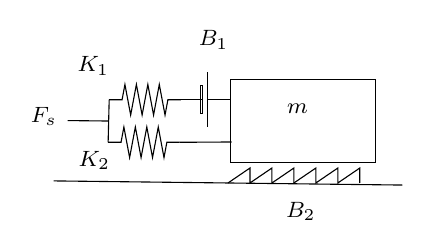
\begin{tikzpicture}[x=0.75pt,y=0.75pt,yscale=-1,xscale=1]
%uncomment if require: \path (0,131); %set diagram left start at 0, and has height of 131

%Straight Lines [id:da6572736986020198] 
\draw    (25.5,85.96) -- (193.5,87.96) ;
%Shape: Rectangle [id:dp37179193982442404] 
\draw   (110.5,37) -- (180.5,37) -- (180.5,77) -- (110.5,77) -- cycle ;
%Shape: Resistor [id:dp5863255716244715] 
\draw   (51.75,67.36) -- (57.96,67.36) -- (59.34,60) -- (62.1,74.71) -- (64.86,60) -- (67.62,74.71) -- (70.38,60) -- (73.14,74.71) -- (75.9,60) -- (78.66,74.71) -- (80.04,67.36) -- (86.25,67.36) ;
%Shape: Resistor [id:dp9559934425910204] 
\draw   (52.25,46.86) -- (58.46,46.86) -- (59.84,39.5) -- (62.6,54.21) -- (65.36,39.5) -- (68.12,54.21) -- (70.88,39.5) -- (73.64,54.21) -- (76.4,39.5) -- (79.16,54.21) -- (80.54,46.86) -- (86.75,46.86) ;
%Shape: Battery [id:dp14150408217983101] 
\draw   (86.75,46.86) -- (97.33,46.86) (99.68,33.5) -- (99.68,60.21) (99.68,46.86) -- (110.25,46.86) (96.39,40.18) -- (97.33,40.18) -- (97.33,53.53) -- (96.39,53.53) -- (96.39,40.18) -- cycle ;
%Straight Lines [id:da9821031298071496] 
\draw    (111.25,67.21) -- (86.25,67.36) ;
%Straight Lines [id:da8009331311825136] 
\draw    (52.25,46.86) -- (51.75,67.36) ;
%Straight Lines [id:da15421474776017385] 
\draw    (32.25,56.89) -- (52,57.11) ;
%Shape: Sawtooth Wave Form [id:dp33023020577621964] 
\draw   (109.5,86.96) -- (120.08,79.75) -- (120.08,86.96) -- (130.67,79.75) -- (130.67,86.96) -- (141.25,79.75) -- (141.25,86.96) ;
%Shape: Sawtooth Wave Form [id:dp7198605294026317] 
\draw   (141.25,86.96) -- (151.83,79.75) -- (151.83,86.96) -- (162.42,79.75) -- (162.42,86.96) -- (173,79.75) -- (173,86.96) ;


% Text Node
\draw (13.25,49.4) node [anchor=north west][inner sep=0.75pt]  [font=\footnotesize]  {$F_{s}$};
% Text Node
\draw (136.75,47.4) node [anchor=north west][inner sep=0.75pt]  [font=\footnotesize]  {$m$};
% Text Node
\draw (94.25,12.4) node [anchor=north west][inner sep=0.75pt]  [font=\footnotesize]  {$B_{1}$};
% Text Node
\draw (136.25,94.9) node [anchor=north west][inner sep=0.75pt]  [font=\footnotesize]  {$B_{2}$};
% Text Node
\draw (36.25,70.4) node [anchor=north west][inner sep=0.75pt]  [font=\footnotesize]  {$K_{2}$};
% Text Node
\draw (35.75,24.9) node [anchor=north west][inner sep=0.75pt]  [font=\footnotesize]  {$K_{1}$};


\end{tikzpicture}

\end{document}